\begin{figure}[h]%
\label{fig11}%
\centering
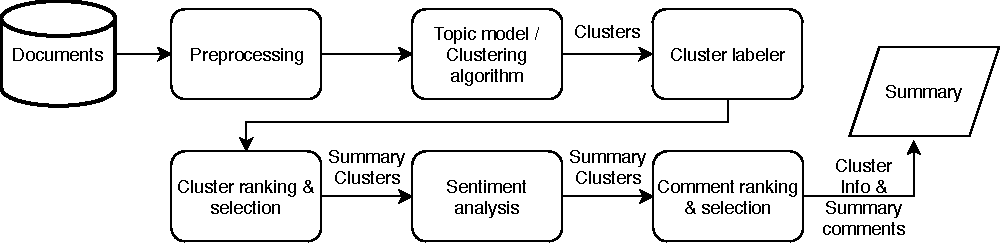
\includegraphics[width=0.95\textwidth]{img/overall_approach1.pdf}
\caption{Outline of the approach used for summary generation.}%
\end{figure}
In the previous section we saw that there are plenty of methods for extractive sumarization. However, there is a common denominator \cite{DBLP:books/sp/mining2012/NenkovaM12}, a three-step approach which is also found in related works targeting single-article comment summarization \cite{DBLP:conf/cikm/MaSYC12, llewellyn_grover_oberlander, DBLP:conf/ecir/FunkABPHG17}.
The same three-step approach consisting of topic clustering, ranking and selection is used in this thesis. The definition of \hyperref[tcdef]{topic clustering} from \hyperref[background]{section 2} shall be refined for our chosen approach in the following.
\begin{enumerate}
\item \textbf{Topic clustering} - In this step, we cluster comments by their topic. Hard clustering is performed, where each comment belongs to exactly one cluster, which tackles data sparsity \cite{DBLP:journals/tacl/NguyenBDJ15}. Each comment is assigned to its most significant topic. Topics have a distribution over documents, so that we can express the cluster of each topic $t_i \in T$ as the comments $c \in C$ for which $t_i$ is most likely.
\begin{equation}
C^{t_i} = \left\{c \in C| t_i = \argmax_{t \in T} P(t|c)\right\}
\end{equation}
In order to cluster comments by topic, we compare the topic models HMDP and LDA and the graph-clustering algorithm MCL.
\item \textbf{Ranking of comments and clusters} - Ranking comments establishes how significant a comment is in respect to its topic. Therefore, comments are only ranked within each topic cluster found in the previous step.
As outlined in \hyperref[rankingdef]{section 2}, ranking bases on a scoring function and a linear order relation. Each cluster is ranked based on the number of comments contained in it and each comment within a cluster is ranked based on its Maximal Marginal Relevance. A higher score indicates a higher significance.
\item \textbf{Selection} The ten highest ranked clusters and their highest ranked comment of each positive and negative sentiment are selected as summary.
\end{enumerate} 
Selection requires the sentiment of a comment to be known. Therefore, we use sentiment analysis before selection.
Furthermore, a short label is given to each topic cluster after topic modeling and clustering.
In the following, the tasks of topic modeling and clustering are described in detail. Later stages of summary generation, namely ranking, sentiment analysis, selection and visualization can be found in \autoref{sumgen}. \par
This thesis and the following sections focus on topic clustering, since the challenges of an unknown number of topics and topics overlapping across comment sections of different articles are significant in multi-article summarization. Moreover, we want to target the problem of data sparsity with context inclusion in the HMDP.

\subsection{Data source}
In order to execute the outlined approach, we considered different datasets upon their fulfillment of domain and metadata requirements as follows.
\begin{itemize}
\item Multiple, topically related, articles.
\item Time of every articles publication.
\item A sufficient number of comments of each article.
\item Metadata for comments:
\begin{itemize}
\item Link between article and comment.
\item Timestamp of publication.
\item Thread identifier.
\end{itemize}
\end{itemize}
Three existing datasets have found consideration.
SoLSCSum \cite{nguyen16} which contains 25,633 comments issued under 157 articles with annotations and gold standard summaries was unavailable as of the start of this thesis.
Second, the SENSEI annotated corpus \cite{DBLP:conf/sigdial/BarkerPAKHG16} contains 18 articles and associated comments from the Guardian newspaper with groupings by topic, based on which human-made summaries were produced. However, the dataset and reference summaries target single-article summarization. Thus, comments are also not grouped across articles which an evaluation of our methods requires.
Therefore, the publicly available Yahoo News Annotated Comments Corpus \cite{napoles2017ynacc} \footnote{\url{https://github.com/cnap/ynacc}} is used throughout this thesis. It contains 522,000 comments issued in 140,000 conversational threads under articles of Yahoo news. Many are topically related on political questions. Furthermore, timestamps and thread identifieres are contained. While articles are not included in the first place, a link of each comment to its article by headline and url exists.
To enforce the constraint of articles being related by topic, three subsets of the YNACC were compiled. Each contain varying amounts of articles and comments to enable a study at different scales. For every article, the content and date of publication was scraped from the website using a rule-based scraper. First, the HTML of each page was retrieved and then, the content within relevant element tags was retrieved using the Python library Scrapy \footnote{\url{https://github.com/scrapy/scrapy}} and its xPath \footnote{\url{https://www.w3.org/TR/xpath/all/}} implementation. Combined with the associated comments from the YNACC, this results in a sufficient dataset. However, as the YNACC does not contain any grouping, one was manually produced as described in \autoref{evalapproach}. In the following, the three subsets are referred to as dataset \#1, dataset \#2 and dataset \#3 ascending by their size for convenience.

\begin{table}[t]
\centering
\caption{Overview over the three YNACC subsets.}
\begin{tabular}{||l||c|c|c||}
\hline
 & {\#}1 & {\#}2 & {\#}3 \\
\hline
No. of articles & 10 & 17 & 38 \\
No. of comment threads & 37 & 46 & 934 \\
No. of comments & 259 & 312 & 6195 \\
Date range & 19/4 - 5/5/2016 & 3/4 - 5/5/2016 & 2/4 - 6/5/2016 \\
Topic domain & narrow & broad & broad \\
\hline
\end{tabular}
\end{table}

\subsection{Characteristics of news article comments}
\label{review}
Now that the skeleton of the approach and datasets are established, we will consider characteristics of news comments in order to be able to formulate sound topic clustering methods. A more thorough evaluation is found in \cite{napoles2017ynacc}.
Therefore, a subset of the YNACC \footnote{\url{https://github.com/cnap/ynacc}} \cite{napoles2017ynacc} annotated by experts is analyzed. It contains 23,383 comments from 696 articles. A list of annotations can be found in the \hyperref[ynacclabel]{Appendix}.
\begin{figure}[h]%
\centering
\subfigure[Boxplot of the no. of words per comment]{%
\label{fig4}%
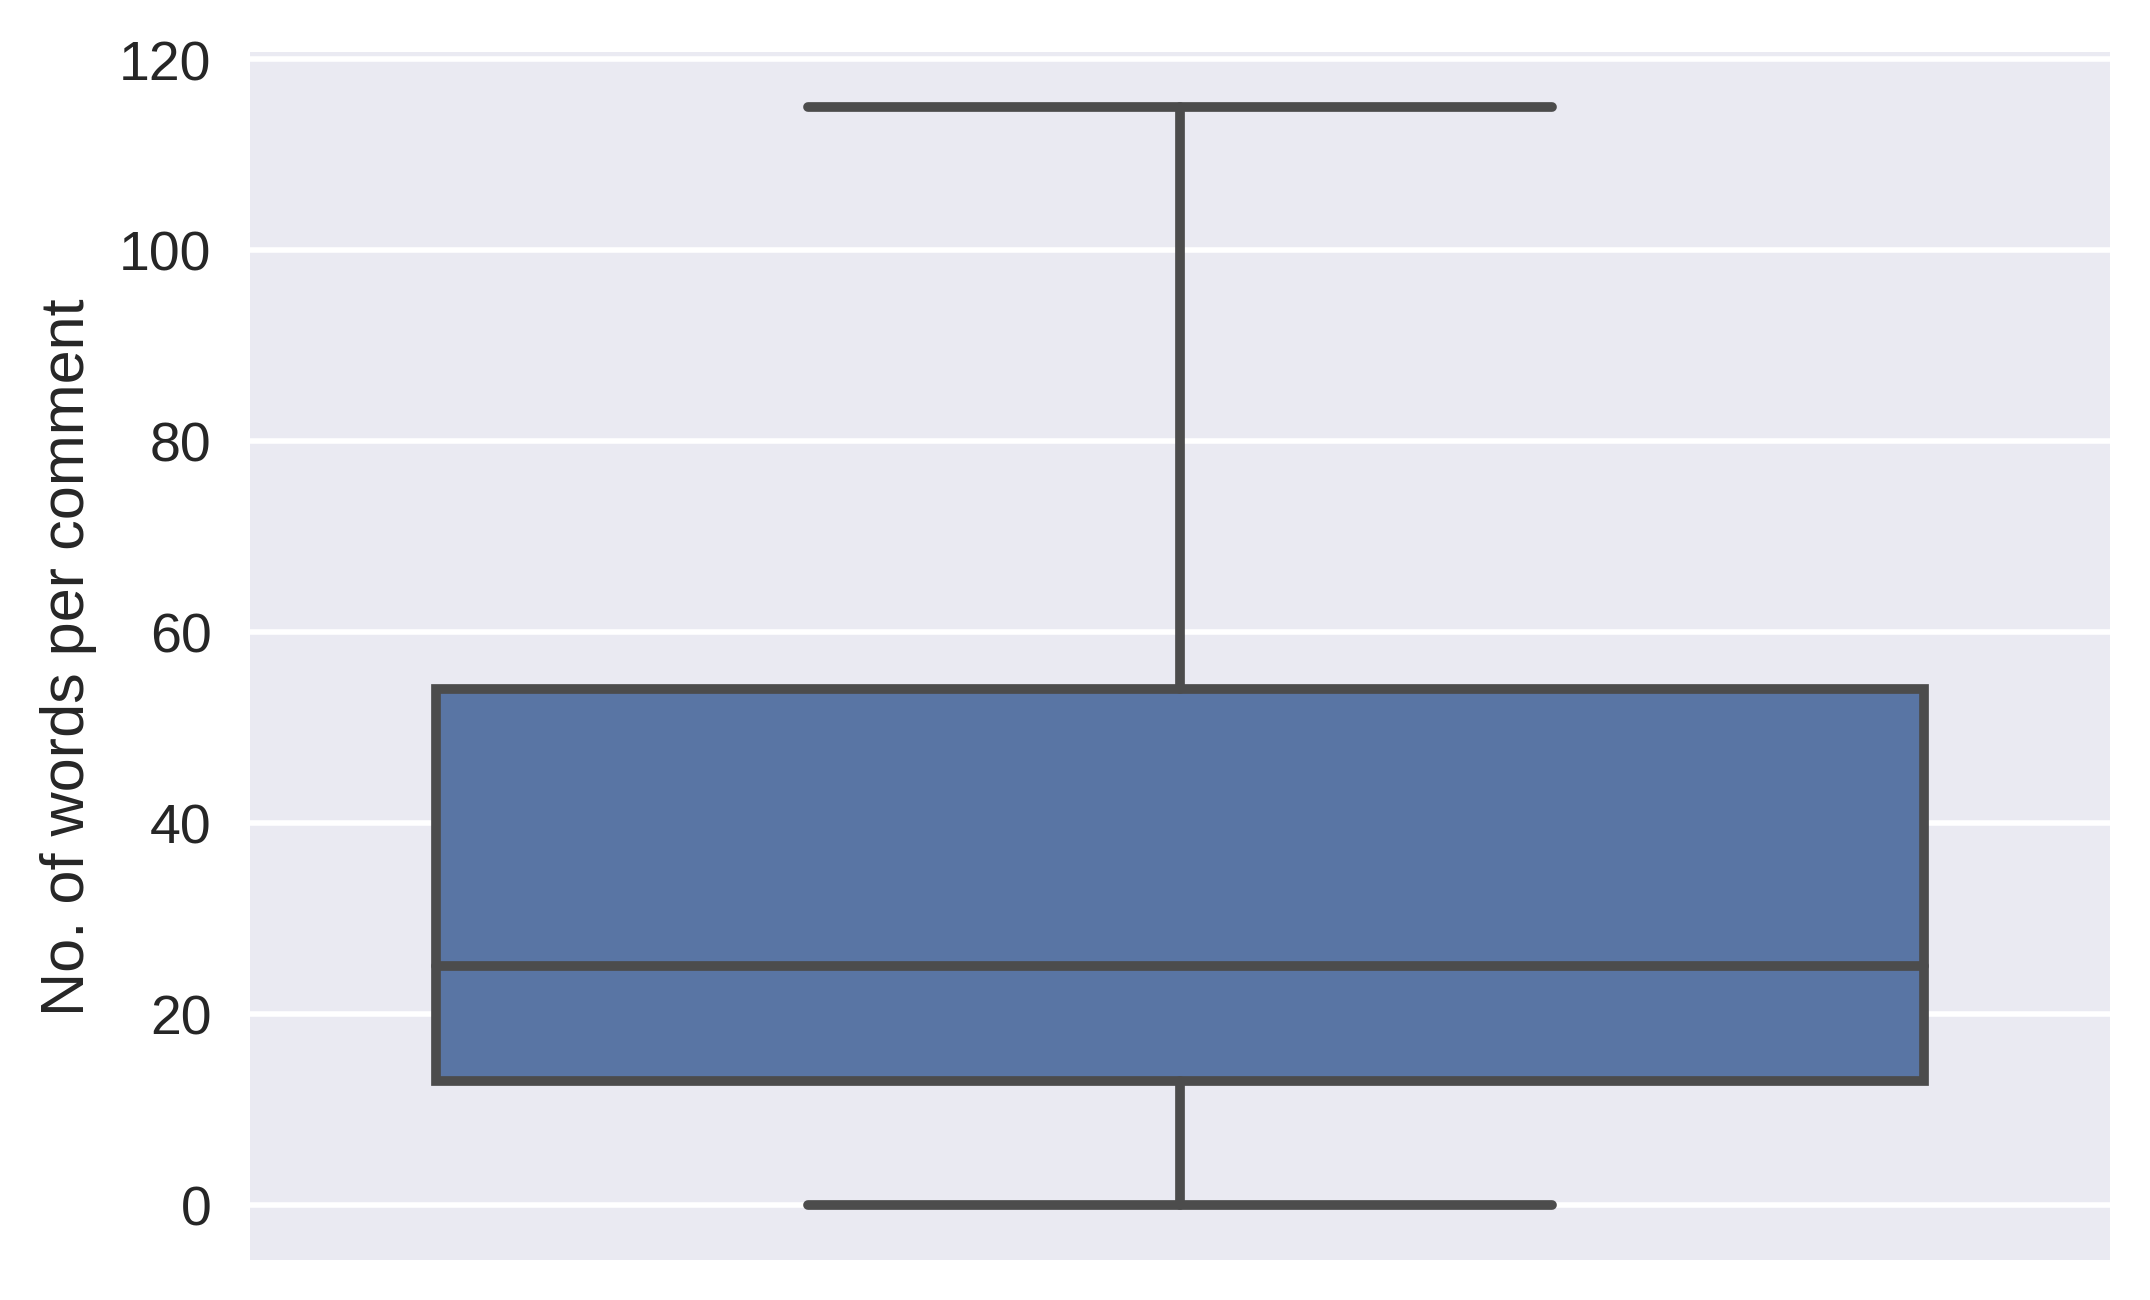
\includegraphics[width=0.45\linewidth]{img/words_expert.png}}%
\qquad
\subfigure[Boxplot of the no. of sentences per comment]{%
\label{fig5}%
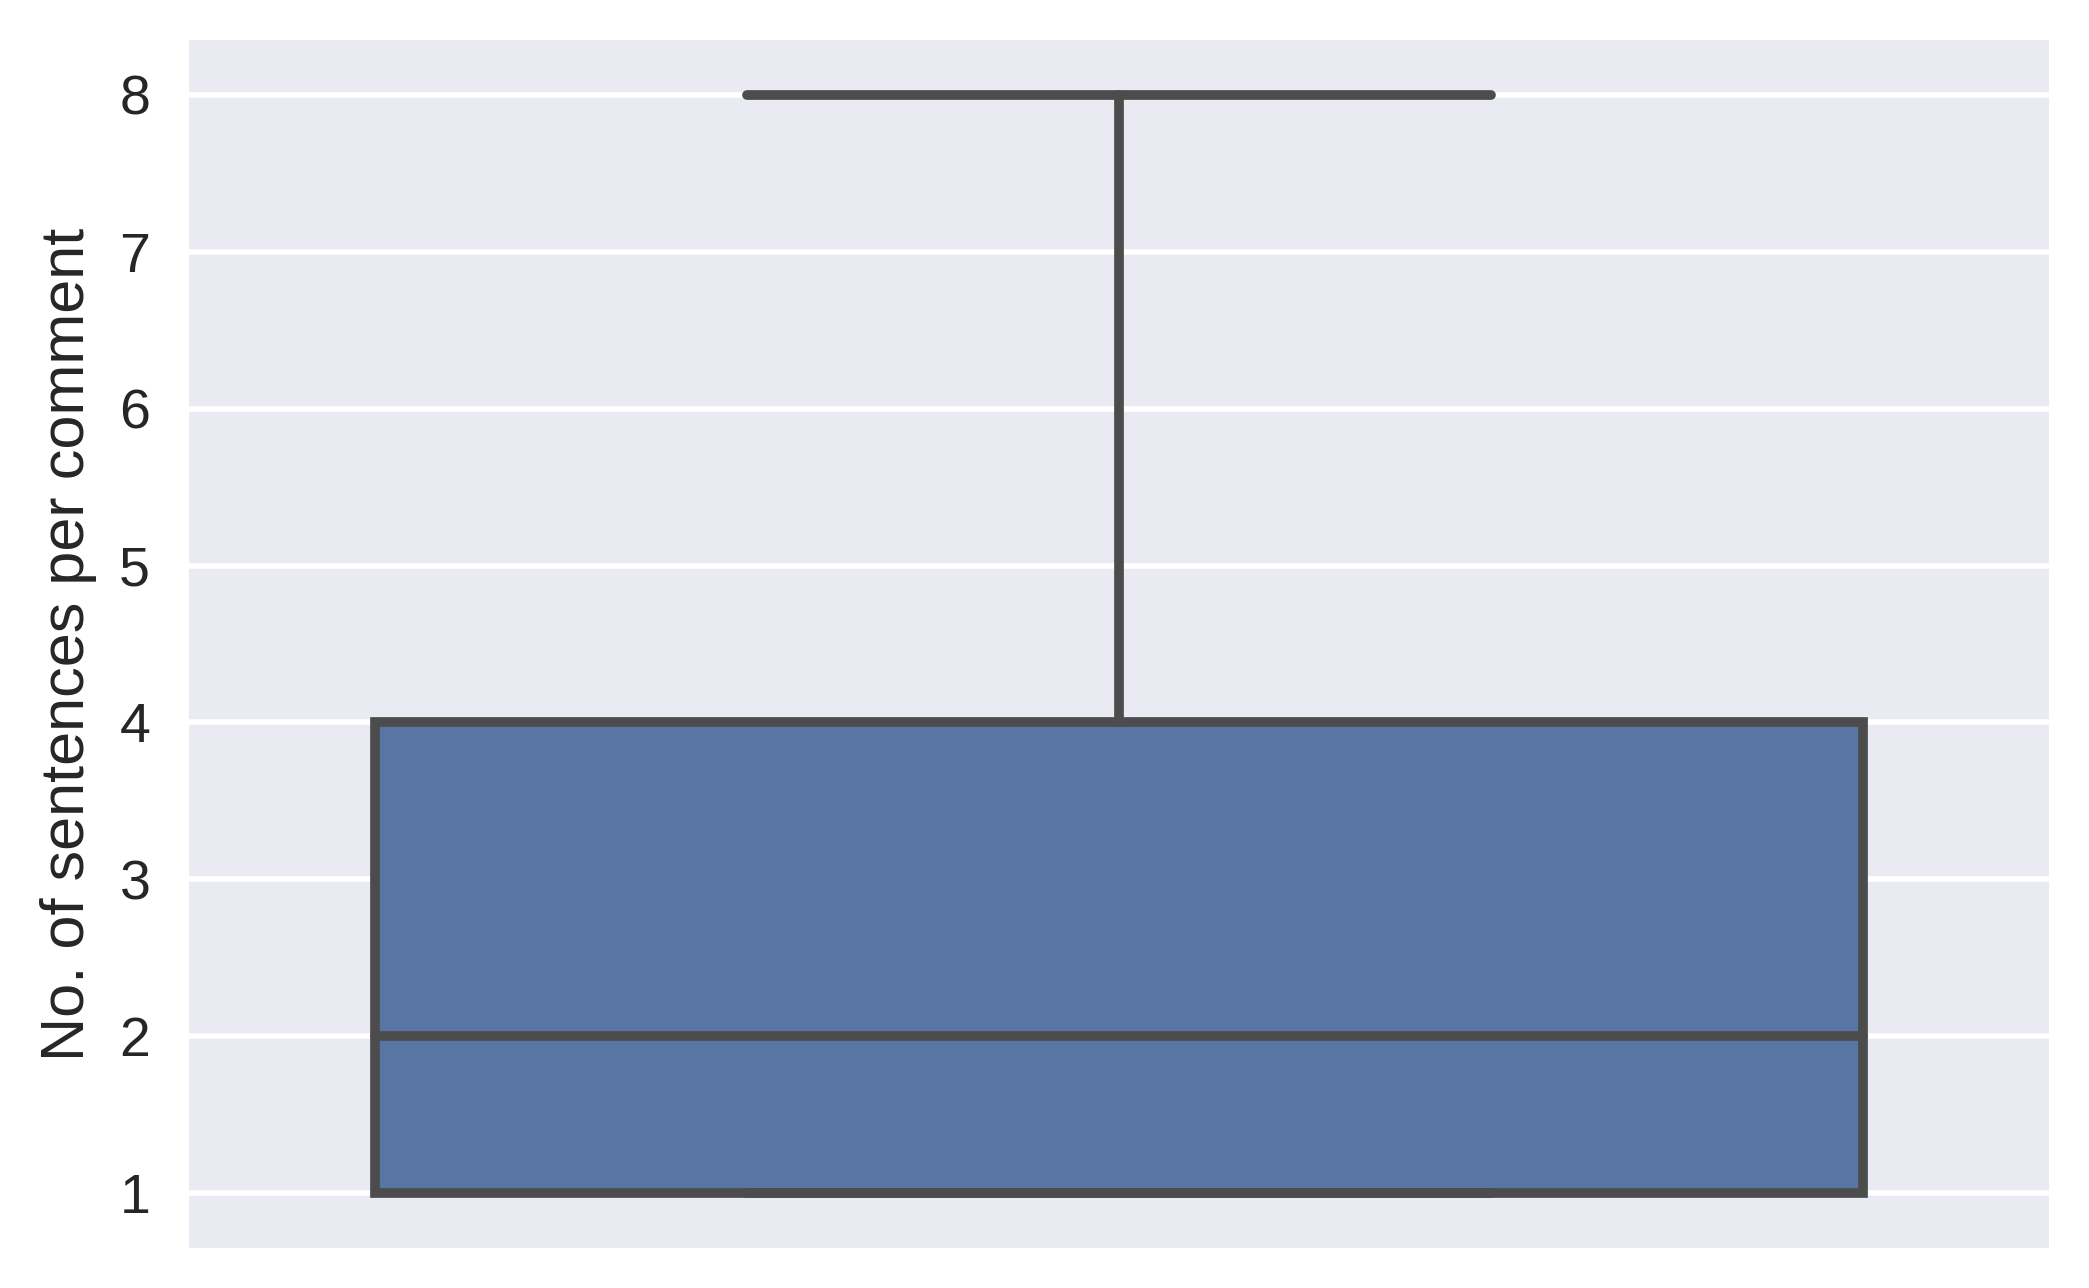
\includegraphics[width=0.45\linewidth]{img/sentences_expert.png}}%
\caption{Description of the comment length for comments in the YNACC subset annotated by experts.}
\end{figure}
\begin{figure}[h]%
\centering
\subfigure[Boxplot of the no. of comments per article]{%
\label{fig6}%
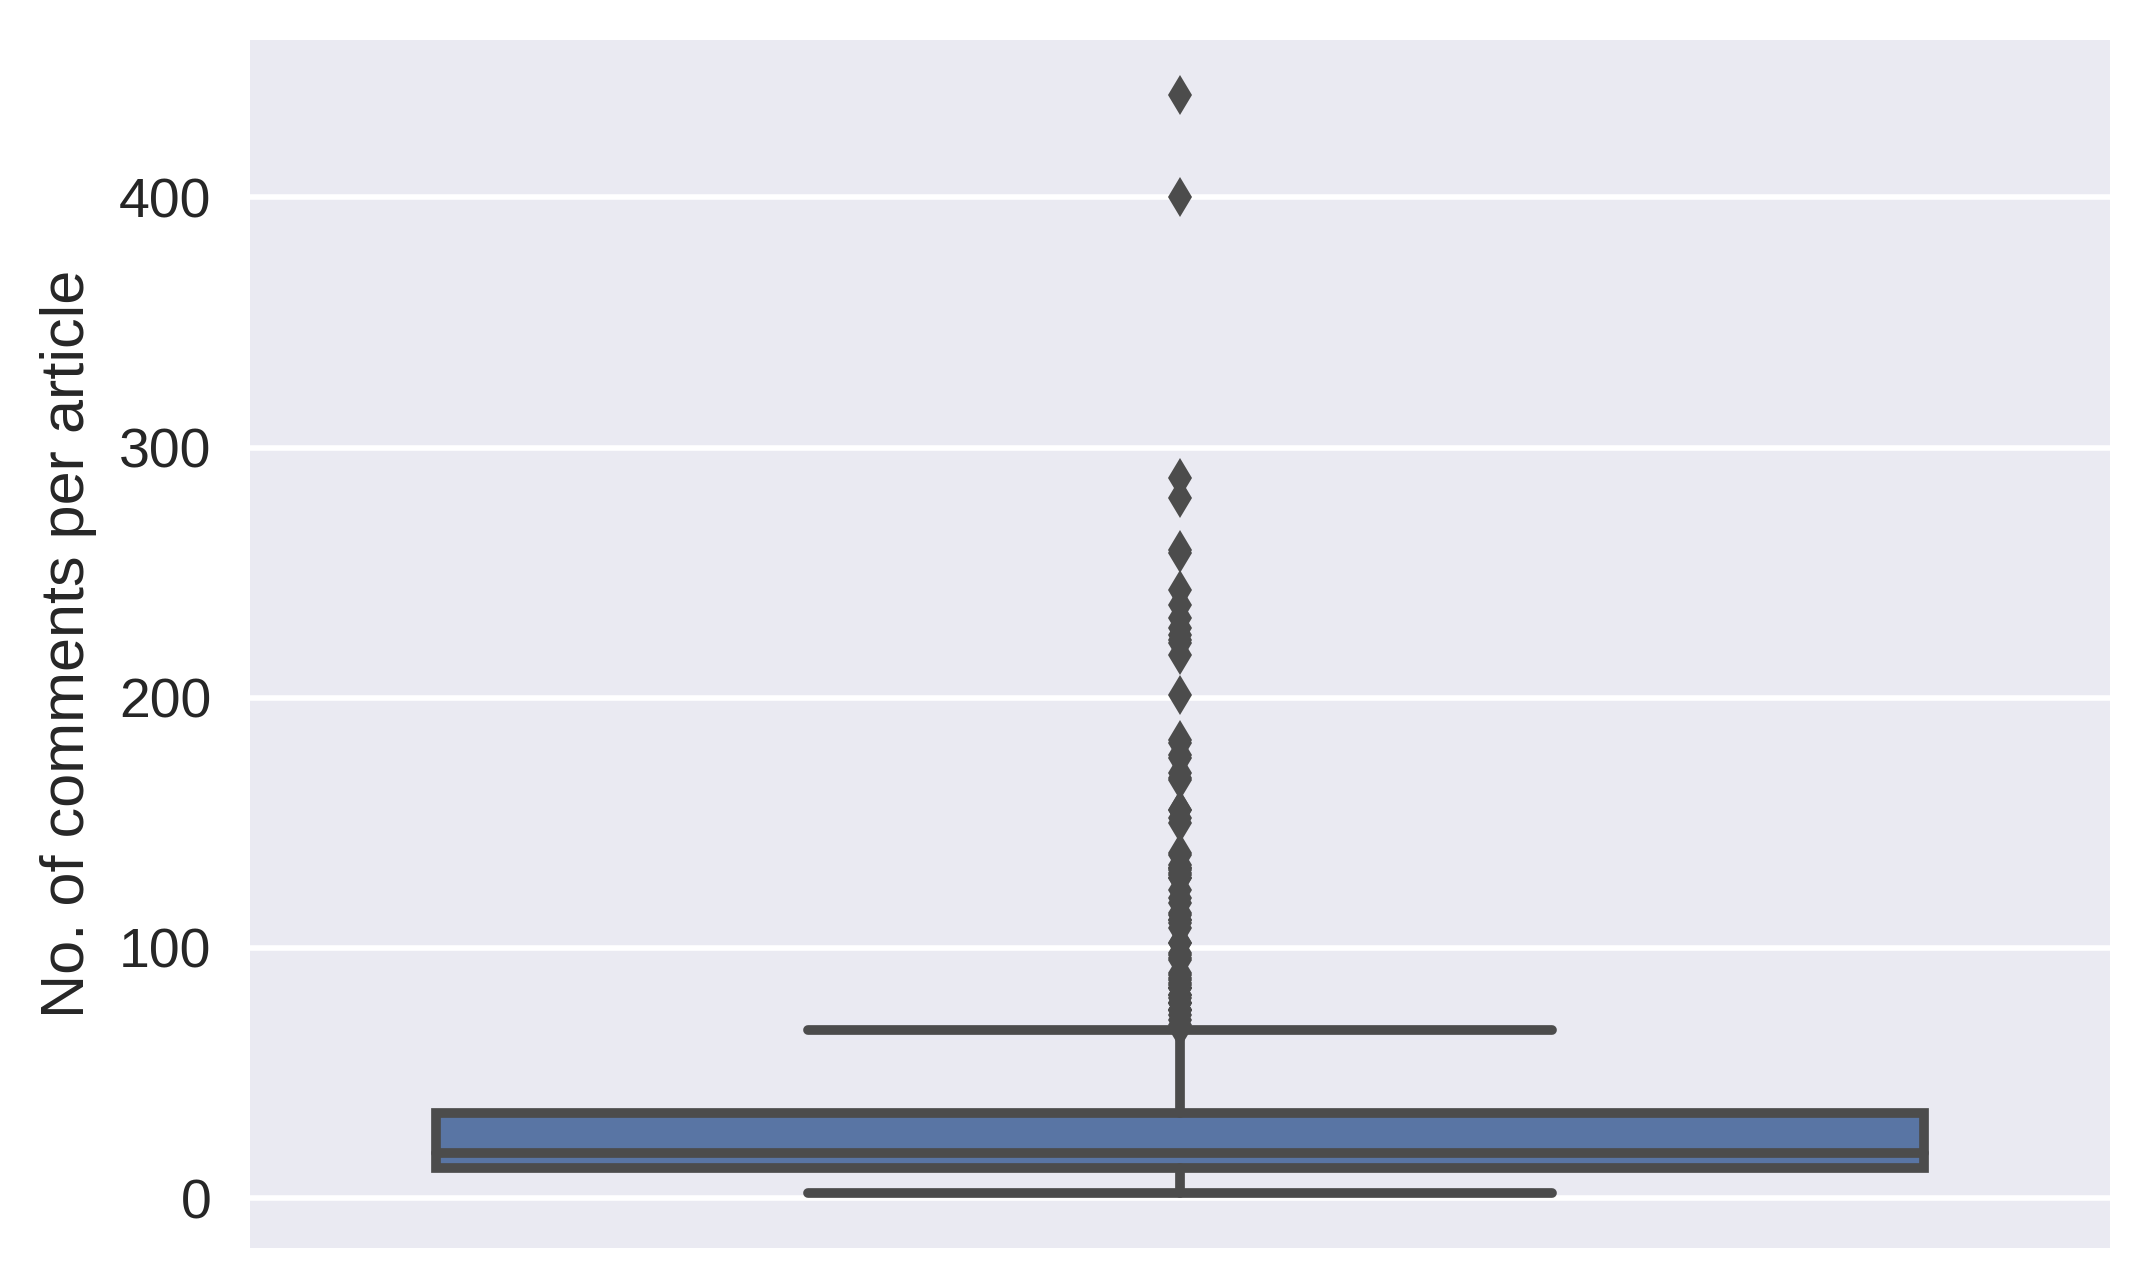
\includegraphics[width=0.45\linewidth]{img/comment_no_article.png}}%
\qquad
\subfigure[Boxplot of the no. of comments per thread]{%
\label{fig7}%
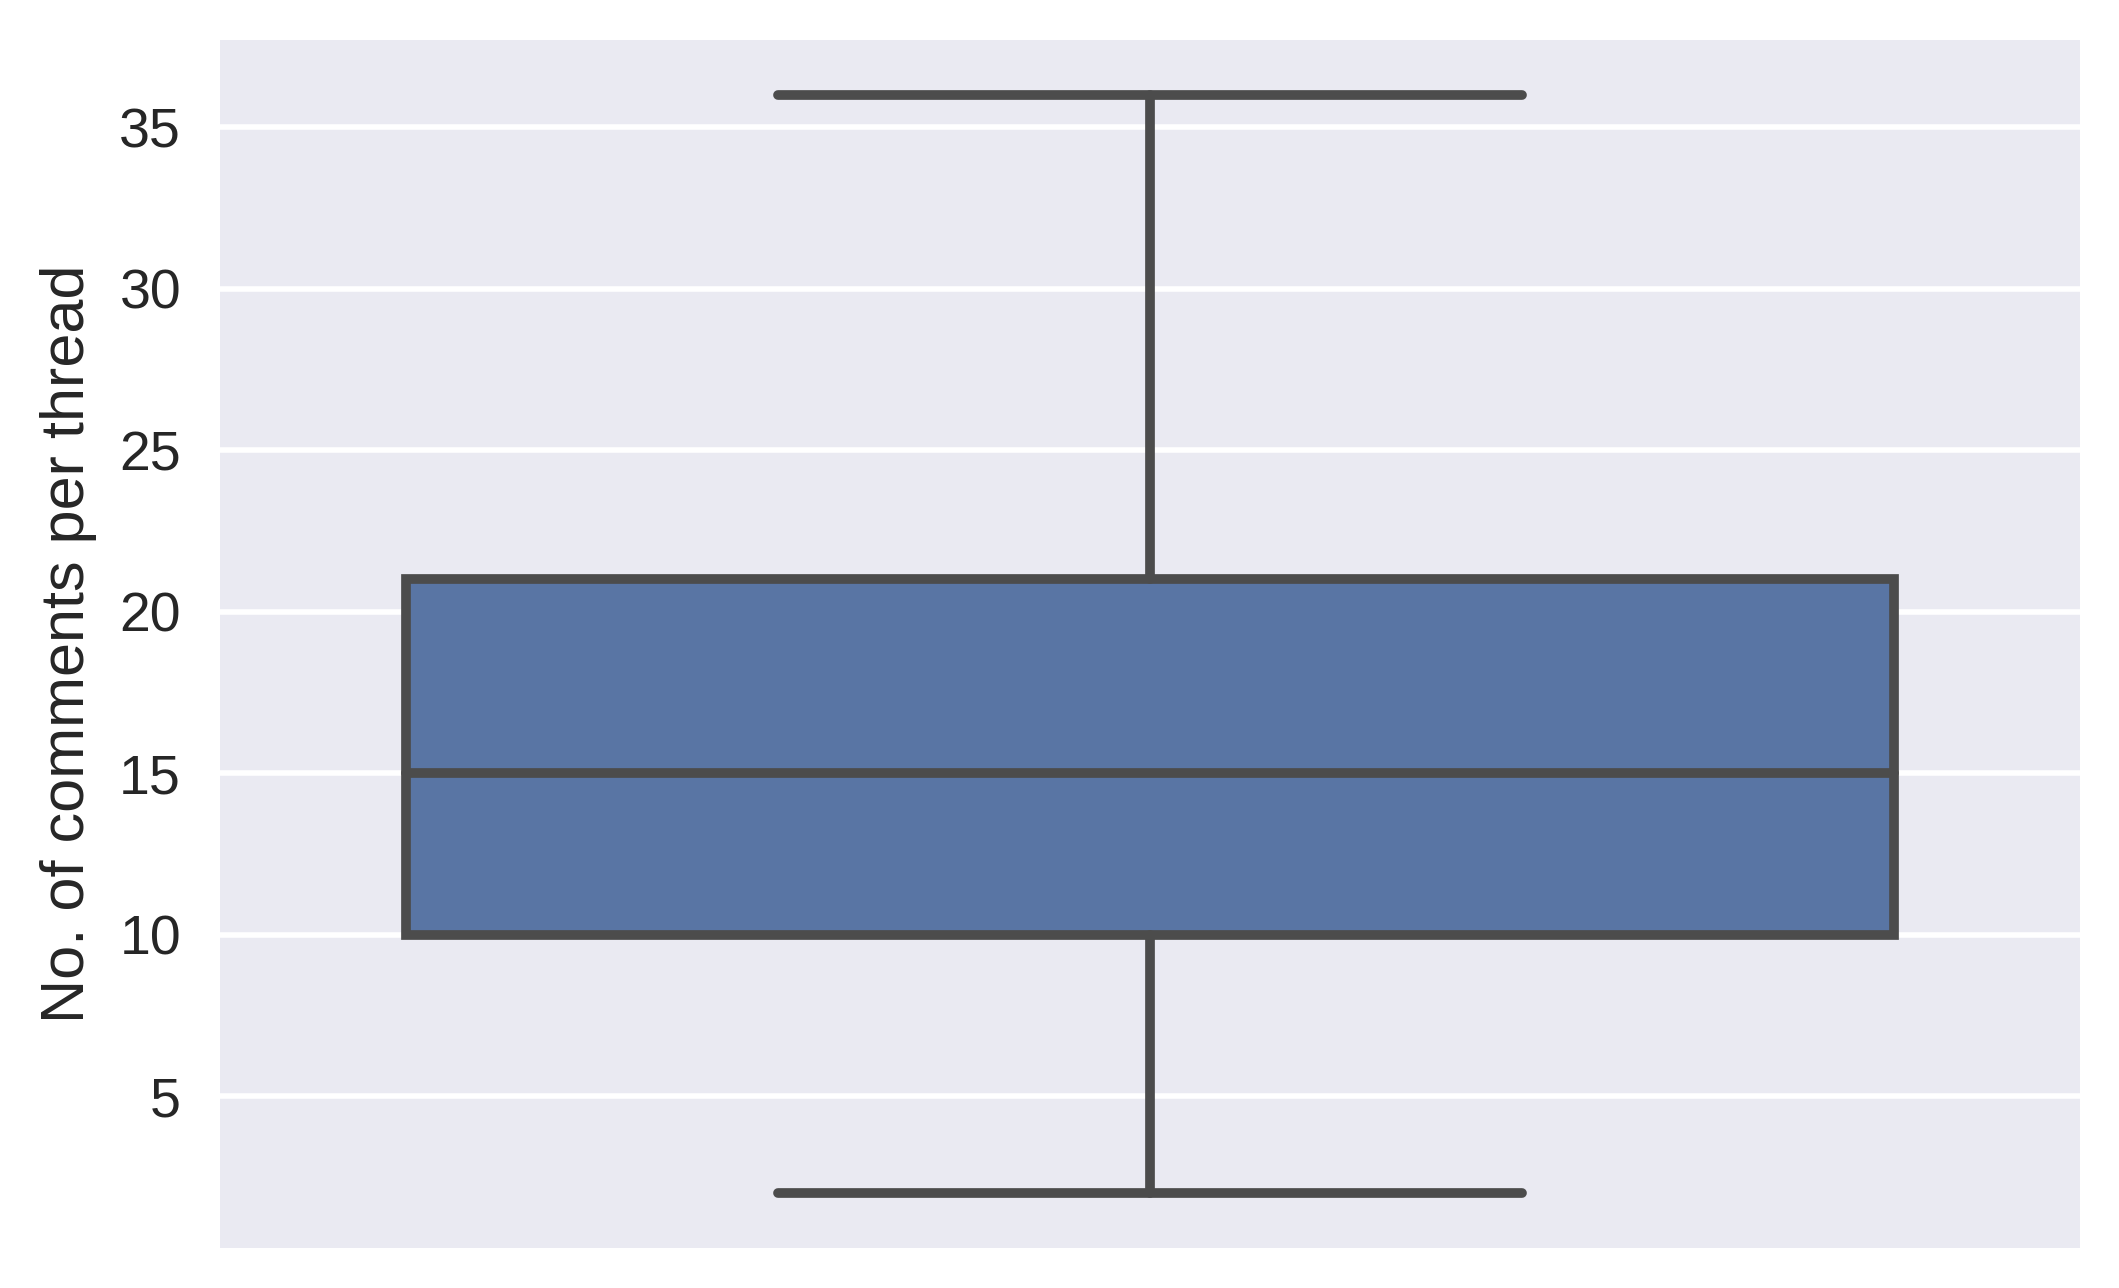
\includegraphics[width=0.45\linewidth]{img/comment_no_thread.png}}%
\caption{No. of comments per article and thread.}
\end{figure}
As outlined in \hyperref[fig4]{Figure 7 a)} and \hyperref[fig5]{b)}, comments are usually short and sparse with a median word count of 25 and a median sentence count of 2. 75\% of comments were not longer than 4 sentences or 54 words. The median vocabulary size of comments is 19 words. Nevertheless, heavy outliers with far more than 100 words exist. The number of comments issued per article fluctuates heavily with a standard deviaton of over 46. In the dataset, each article has between 2 and 441 comments. Comments are grouped in subdialogues which are also called threads and solidify a reply-relationship. Such threads form a significant grouping with a median number of 15 and a maximum number of 48 comments contained.
\begin{figure}[h]%
\centering
\label{fig10}%
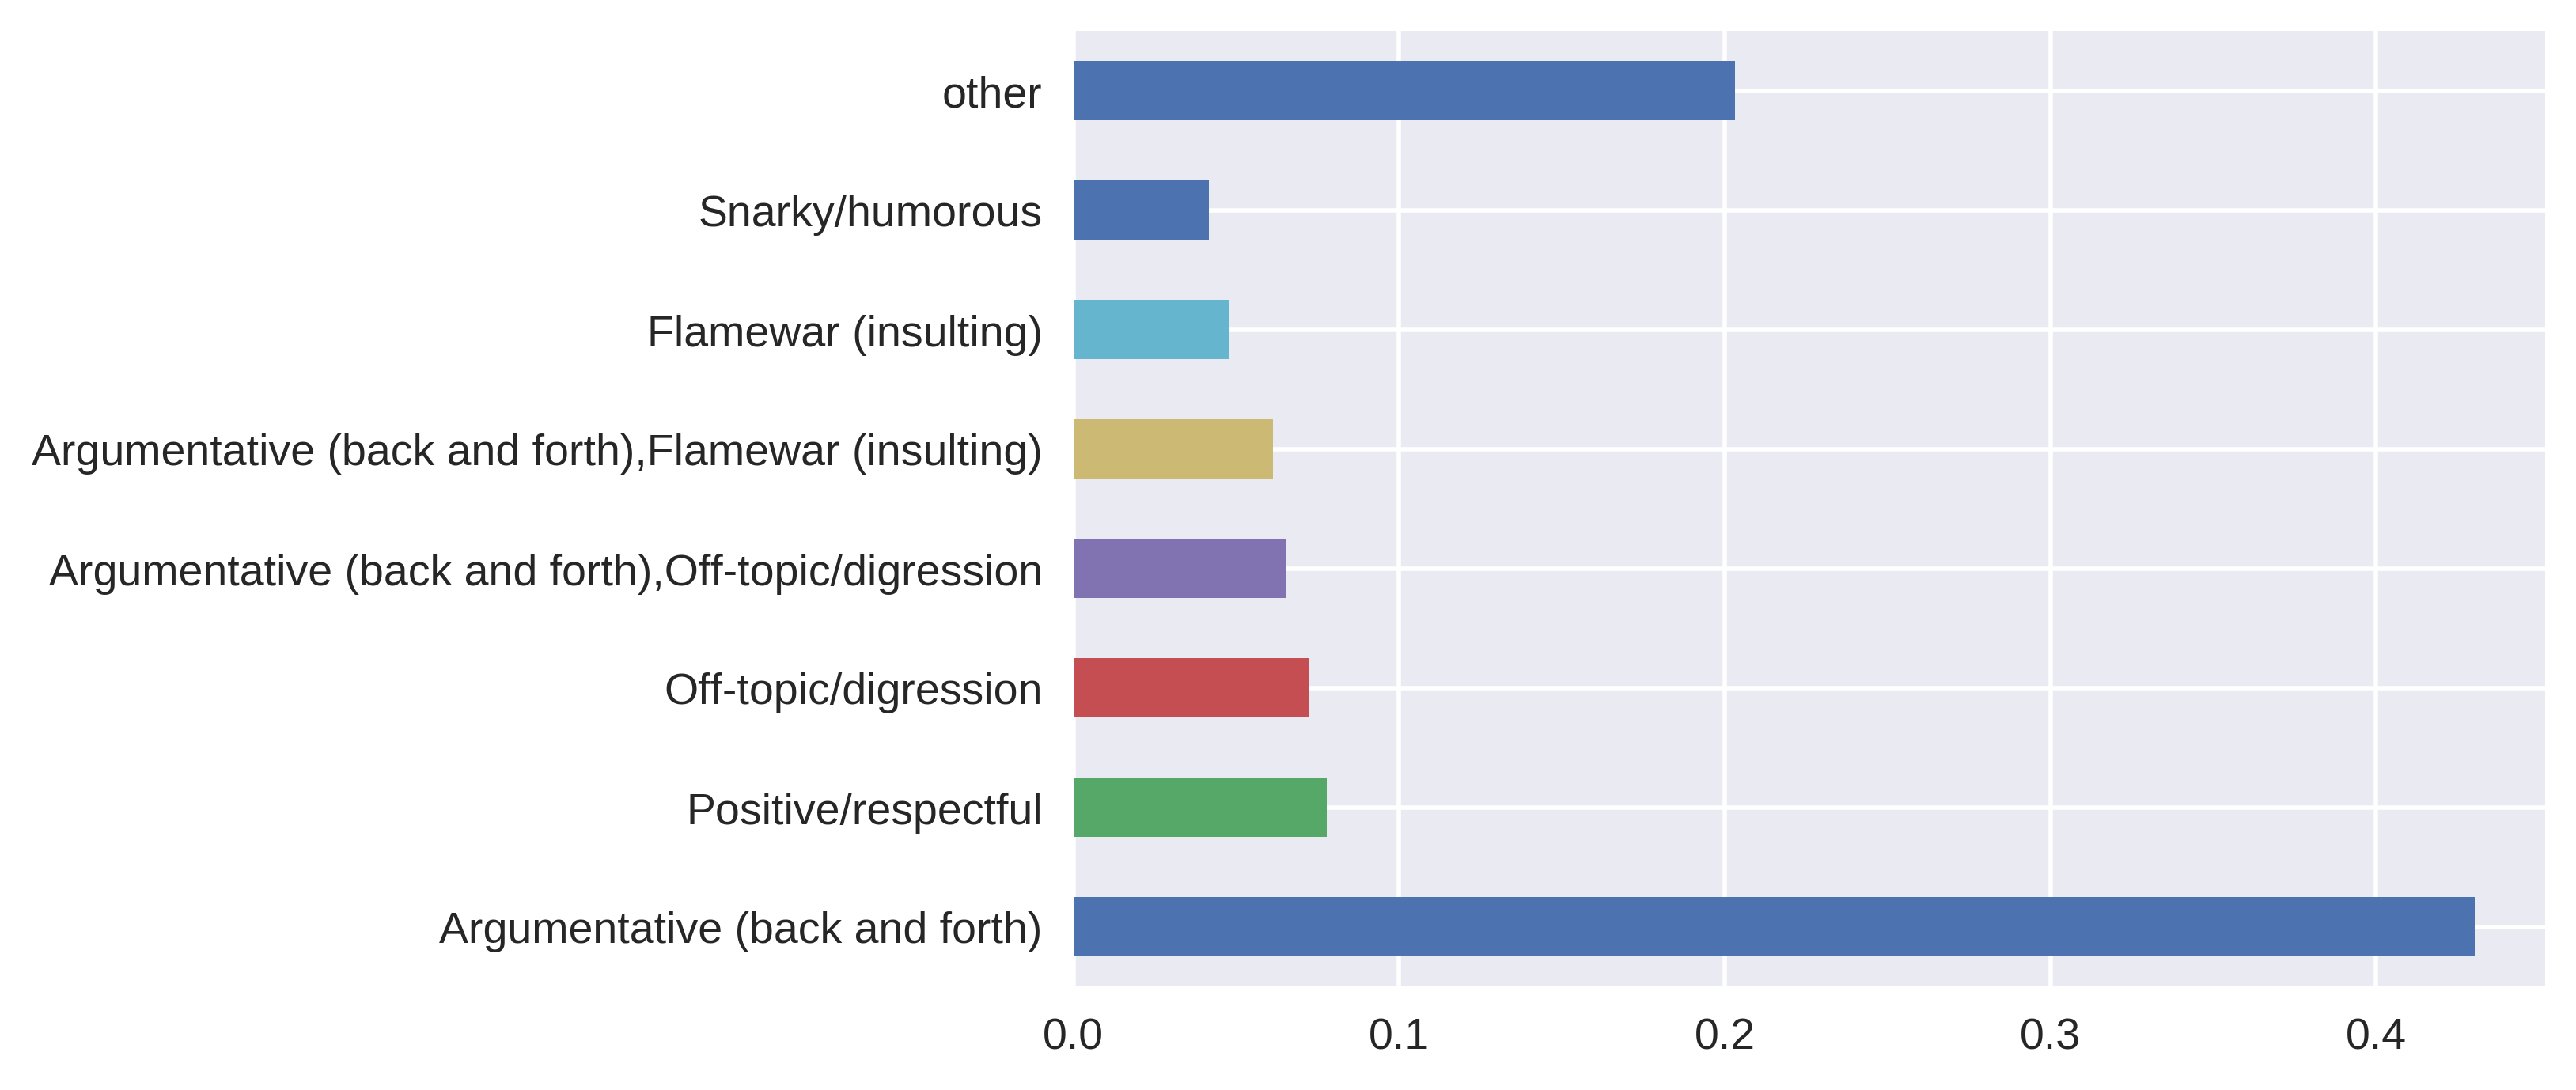
\includegraphics[height=2.5in]{img/convo_type.png}%
\caption{Conversation types within a thread.}%
\end{figure}
A large share of threads contain an argumentative debate, as shown in \hyperref[fig10]{Figure 9}. Typically, such argumentative debates share a common topic. Hence, the thread relationship of two comments can be a determining factor for whether they share a topic. This supports the intra-comment-comment relationship introduced by Ma et al. \cite{DBLP:conf/cikm/MaSYC12}, where comments echo ideas from other comments. The majority of comments is not issued to the general audience but rather as a reply to a specific comment, as outlined in \hyperref[fig9]{Figure 10}, reinforcing the idea that commenters are inspired by other comments.
Nevertheless, such inspiration does not only need to be taken from a comments' article and its commentsphere. Only about 60\% of the comments were labeled as on-topic with the article or illegible of which no distinction was made in the labeling process \footnote{https://github.com/cnap/ynacc/blob/master/rater-guidelines.pdf}. A third of the comments were labeled as off-topic with the article. It is conceivable that a substantial amount of these comments talk about a related topic found in related articles and their comments which make up the relationships inter-comment-comment and inter-news-comment in \cite{DBLP:conf/cikm/MaSYC12}.
Thus, the idea that the conversational structure under comments of topically related articles is very broad with heavily overlapping topics is corroborated. Still, the article of a comment seems to be at least indicative of its topic.

\begin{figure}[h]%
\centering
\label{fig9}%
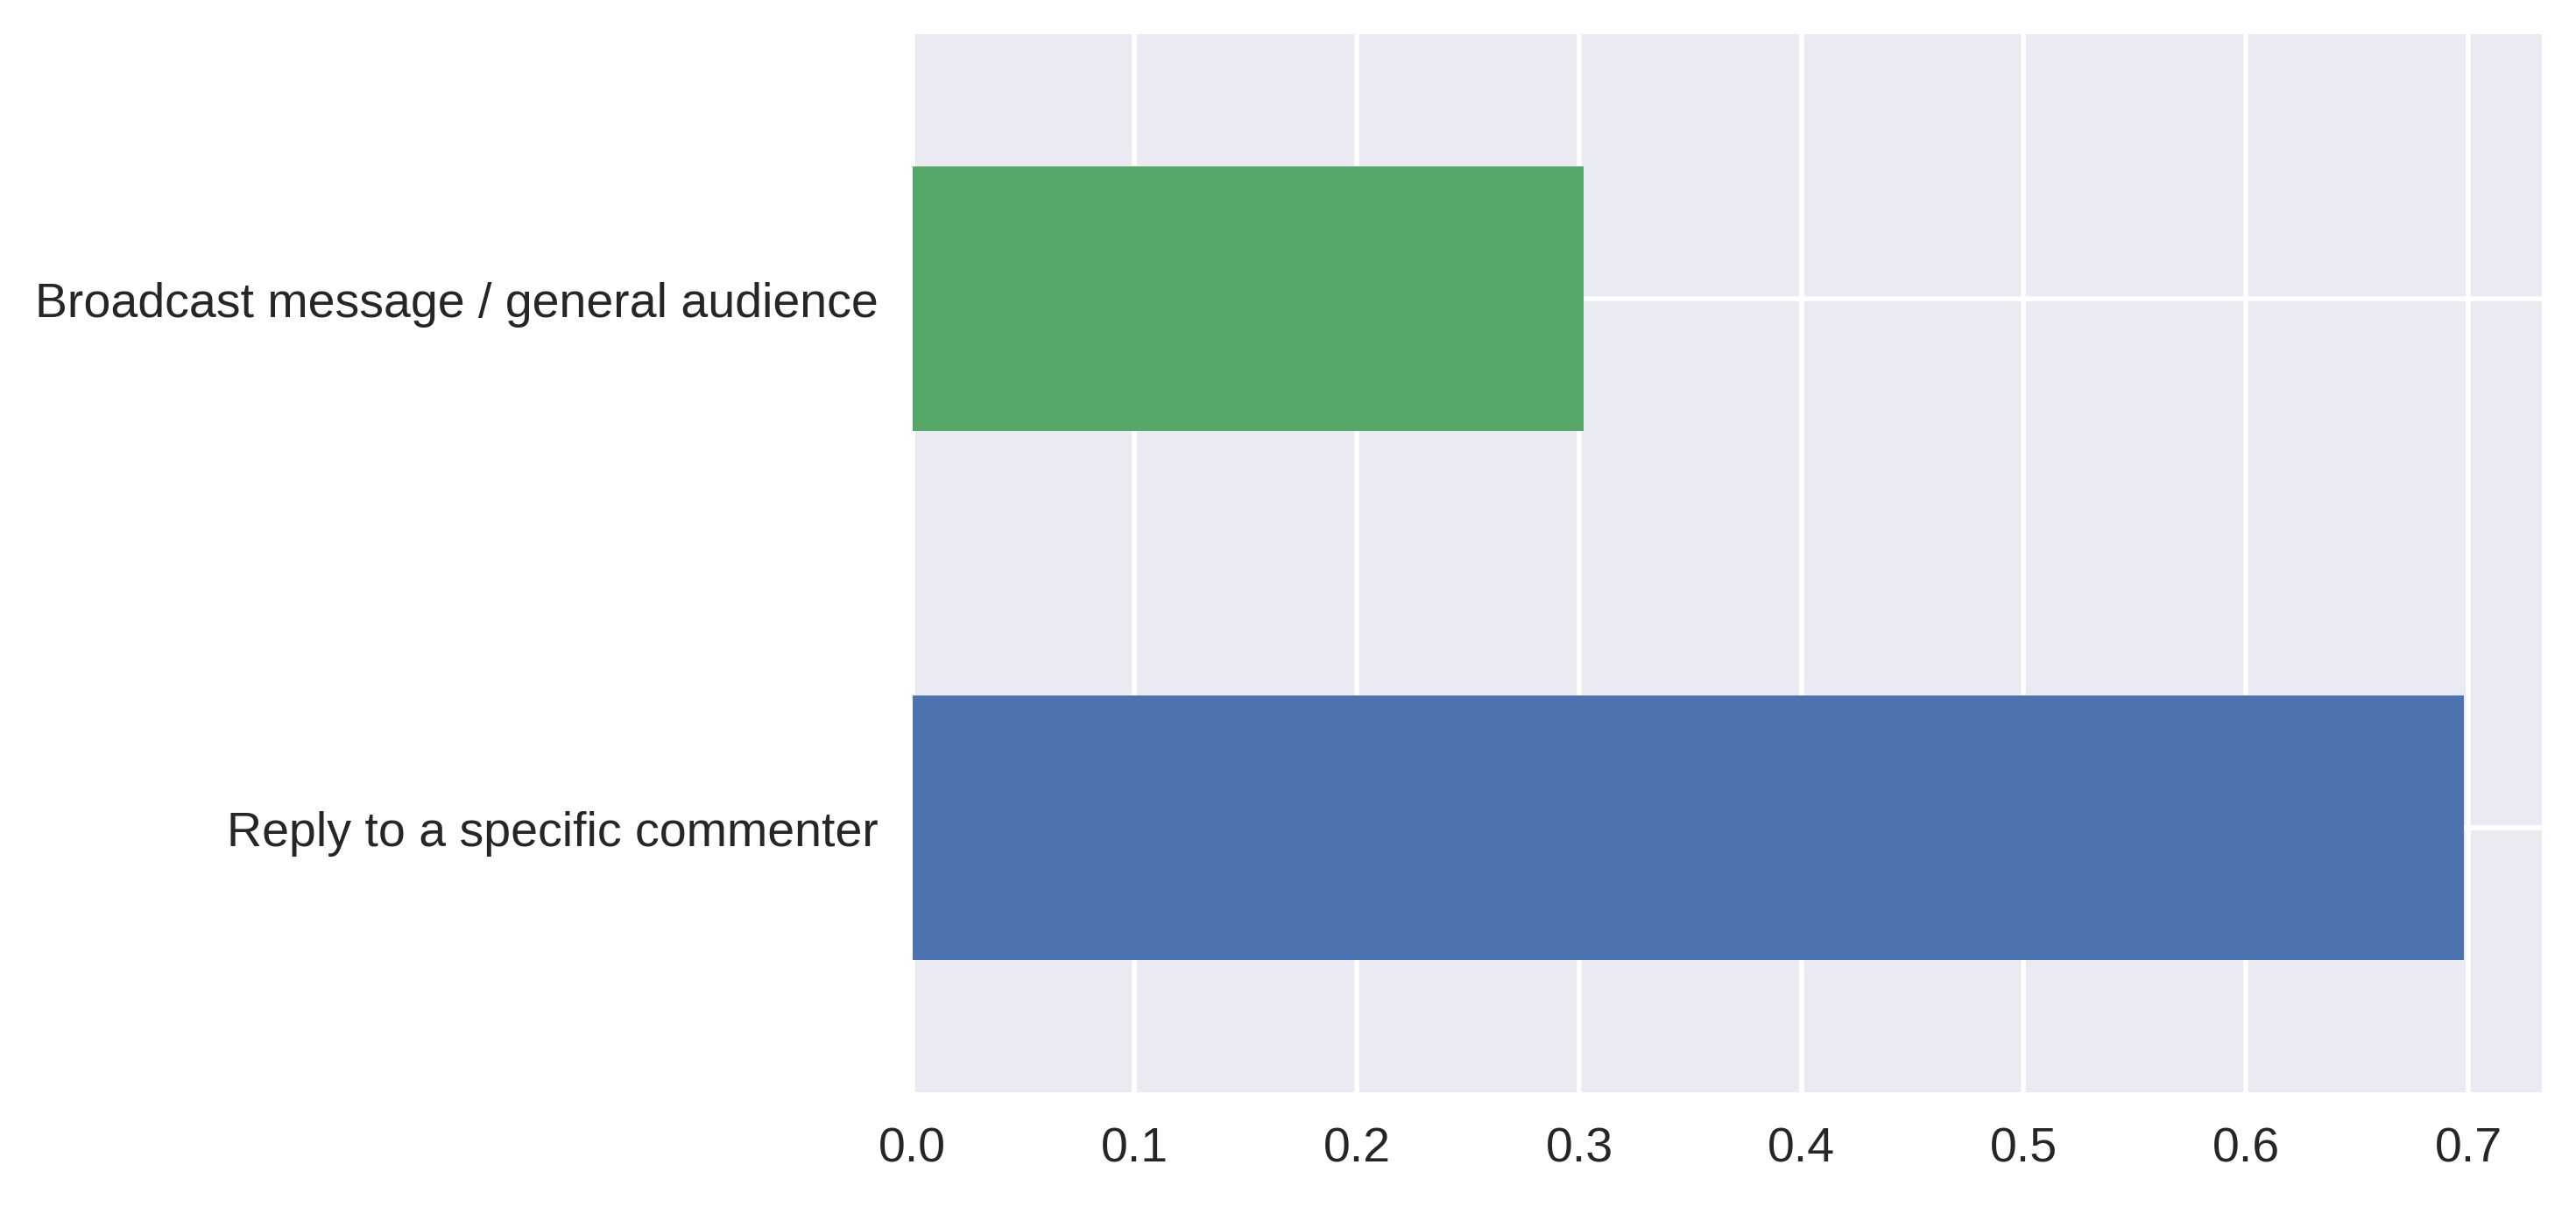
\includegraphics[height=2.5in]{img/audience_expert.png}%
\caption{The intended audience of comments.}%
\end{figure}
\begin{figure}[h]%
\label{fig8}%
\centering
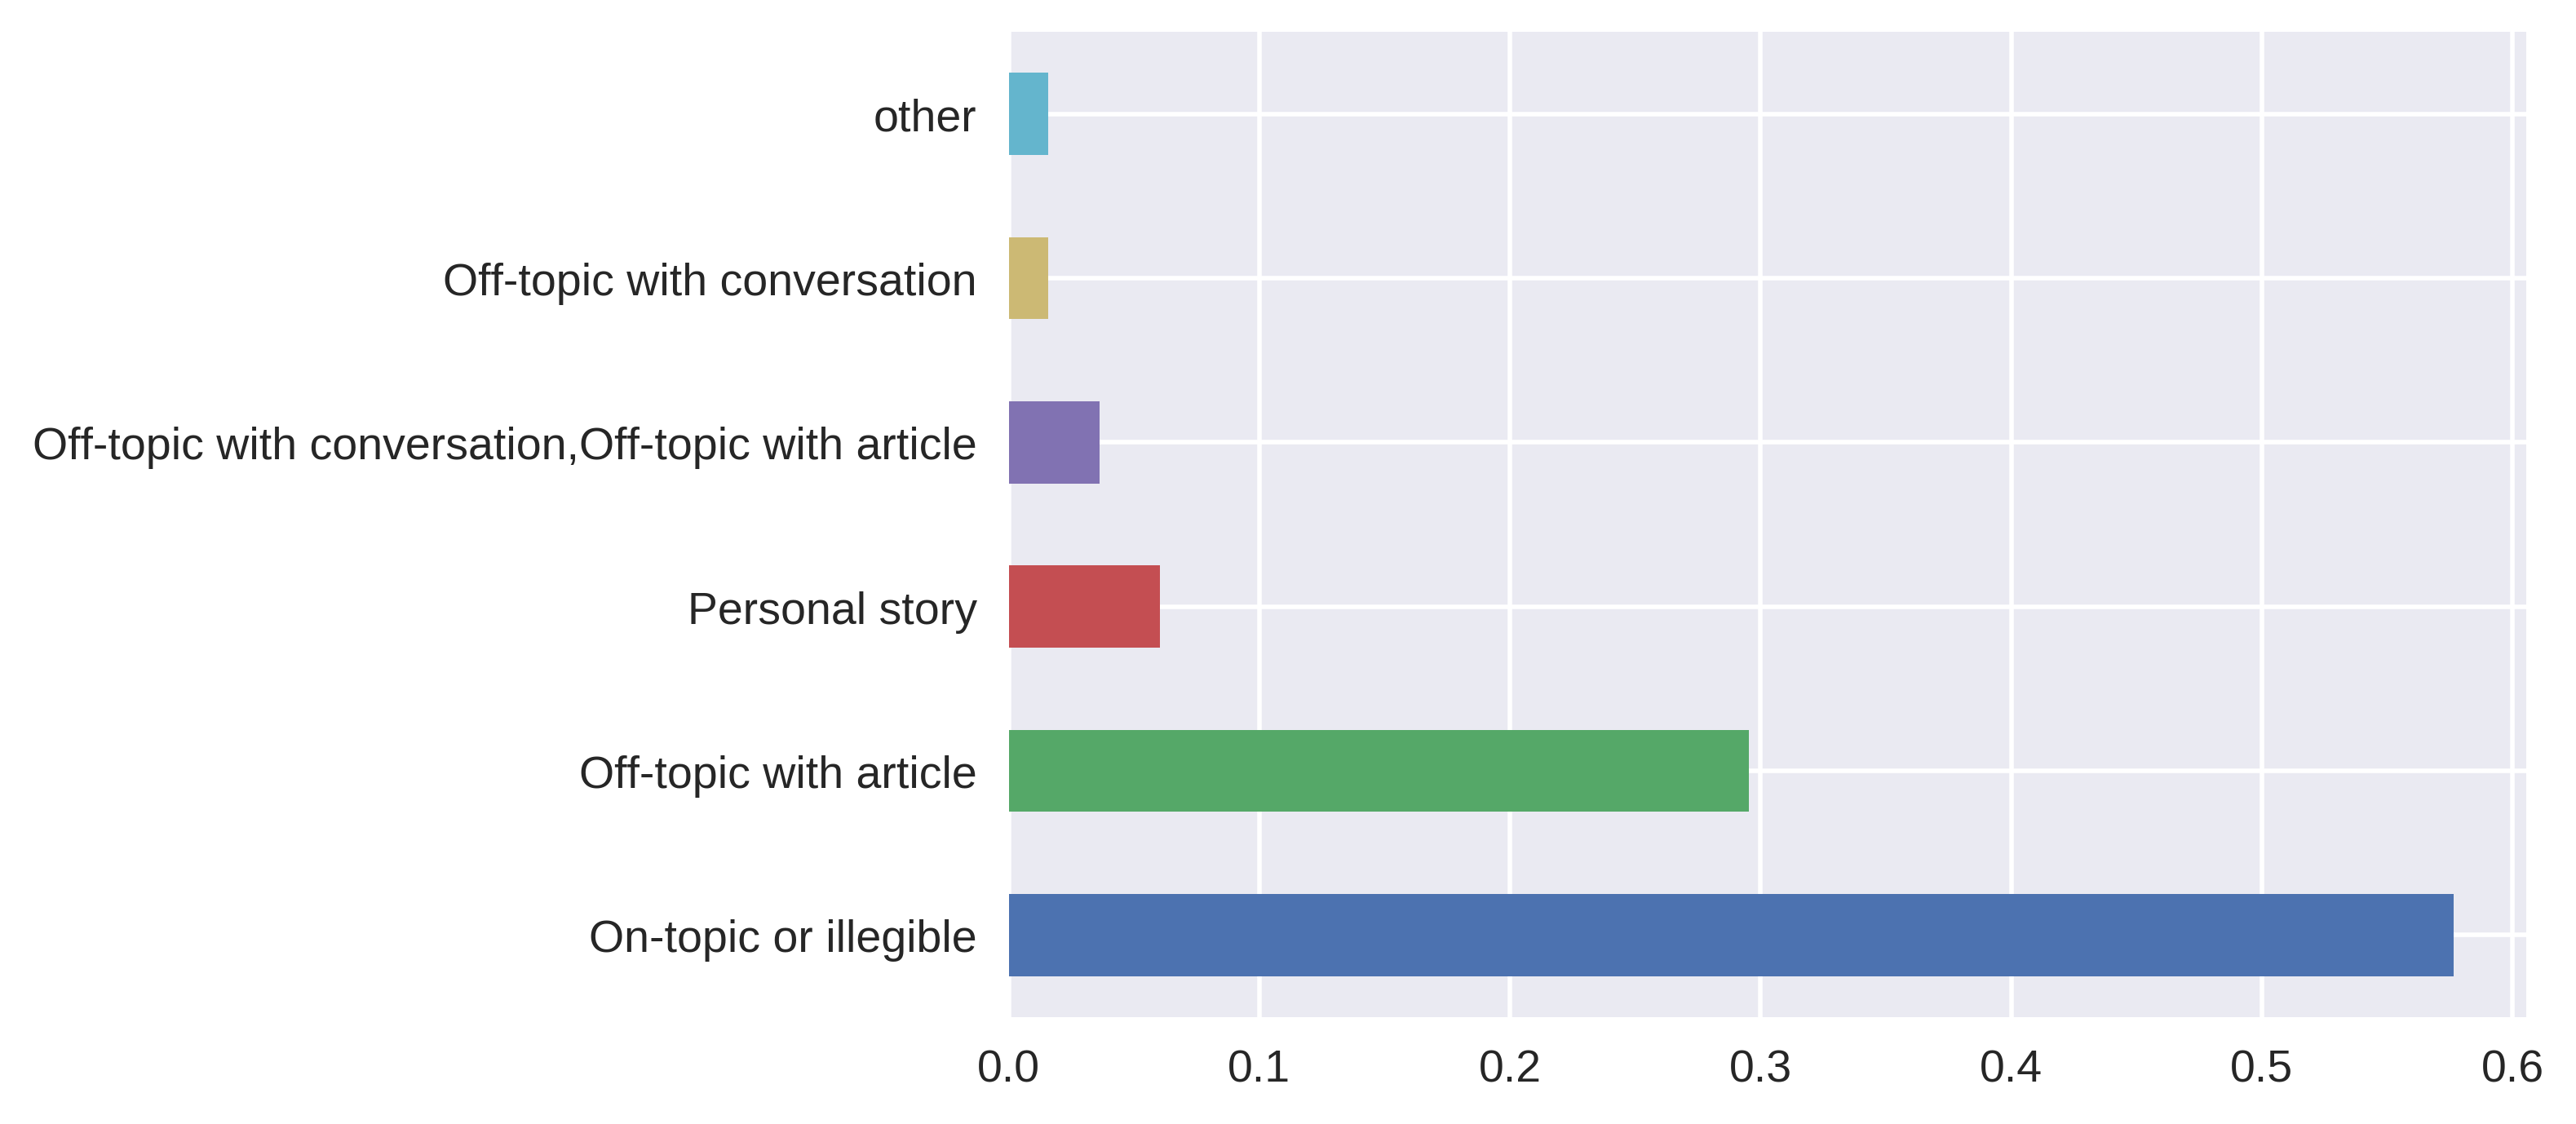
\includegraphics[height=2.5in]{img/pmf_topic_expert.png}
\caption{Topic of comments.}%
\end{figure}

\clearpage